
\documentclass[tikz,border=5pt]{standalone}

\usetikzlibrary{automata, positioning, arrows.meta}

\begin{document}

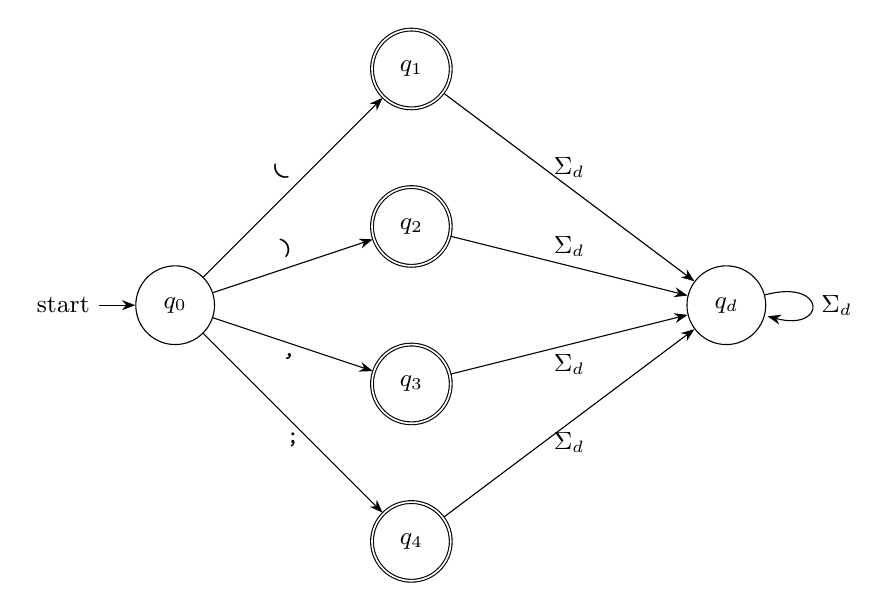
\begin{tikzpicture}[
    ->,
    >=Stealth,
    every state/.style={
        draw,
        circle,
        minimum size=1cm
    },
    font=\small
]


\node[state, initial] (q0) at (0,0) {$q_0$};

\node[state, accepting] (q1) at (3,3) {$q_1$};
\node[state, accepting] (q2) at (3,1) {$q_2$};
\node[state, accepting] (q3) at (3,-1) {$q_3$};
\node[state, accepting] (q4) at (3,-3) {$q_4$};

\node[state] (qd) at (7,0) {$q_d$};


\draw (q0) -- node[above, sloped] {\texttt{(}} (q1);
\draw (q0) -- node[above, sloped] {\texttt{)}} (q2);
\draw (q0) -- node[below, sloped] {\texttt{,}} (q3);
\draw (q0) -- node[below,] {\texttt{;}} (q4);


\draw (q1) to[left=15]
    node[above] {$\Sigma_d$} (qd);

\draw (q2) to[left=8]
    node[above] {$\Sigma_d$} (qd);

\draw (q3) to[left]
    node[below] {$\Sigma_d$} (qd);

\draw (q4) to[left]
    node[below] {$\Sigma_d$} (qd);


\draw (qd) edge[loop right]
    node[right] {$\Sigma_d$} (qd);

\end{tikzpicture}

\end{document}
